The circuit diagram used to calculate $R_c$ is shown in Fig. \ref{fig: non ideal active high}:

\begin{figure}[H]
    \centering
    \begin{minipage}[T]{0.55\textwidth}
        \centering
        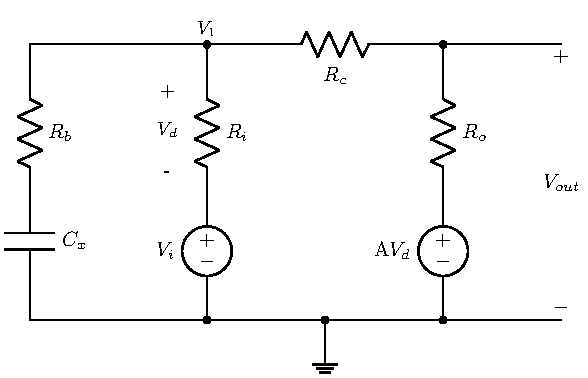
\includegraphics[width=\linewidth]{TU Delft Booming Bass Project Report/figures/PowerAmplifier/circuits/non_ideal opamp circuit.pdf}
        \captionsetup{justification=raggedright, labelfont=bf}
        \caption{The non-ideal equivalent circuit to \autoref{fig: pa active high pass}.}
        \label{fig: non ideal active high}
    \end{minipage}%
    \hspace{0.05\textwidth} % Adjust space between figure and table
    \begin{minipage}[T]{0.35\textwidth}
        \centering
        \begin{tabular*}{0.9\textwidth}{@{\extracolsep{\fill}} c c @{}}
            \toprule
            \textbf{Component} & \textbf{Value of Component} \\
            \midrule
            \textbf{$C_x$} & 79.5$\mu$F \\
            \textbf{$R_b$} & 1k$\Omega$ \\ 
            \textbf{$R_i$} & 200k$\Omega$ \\
            \textbf{$R_o$} & 10$\Omega$ \\
            A & $10^5$ \\
            \bottomrule
        \end{tabular*}
        \captionsetup{justification=raggedright, labelfont=bf}
        \caption{Component values in the non-ideal circuit.}
        \label{tab:ideal values}
    \end{minipage}
\end{figure}







From the circuit, it is clear that the following holds:
\begin{flalign*}
    V_o = 25V_i, \quad V_d = V_1 - V_i
\end{flalign*}
Applying nodal analysis at node $V_1$ in circuit of Fig. \ref{fig: non ideal active high}, gives:
\begin{flalign*}
    \frac{V_{o}-V_{1}}{R_C} + \frac{V_o- 10^5(V_1-V_i)}{R_o} =0 \\
    10(25V_i - V_1) + R_c\left(25V_i - 10^5(V_1 - V_i)\right) = 0 \\
     R_c = -\frac{10(25V_i-V_1)}{25V_i - 10^5V_1 + 10^5V_i} \\
\end{flalign*}

\begin{flalign}
    25V_i + 10^5V_i \approx 10^5 V_i
\end{flalign}

\begin{flalign}
\label{eq: 1}
    R_c = -\frac{25 V_i - V_1}{10^4(V_i-V_1)}
    \equnit{\si{\Omega}}
\end{flalign}


Applying nodal analysis at node 2 gives:
\[\frac{V_1}{R_b + Z_c} + \frac{V_1-V_i}{R_i} + \frac{V_1-V_o}{Rc} = 0\]
\[\frac{V_1 R_c}{R_b + Z_c} + \frac{(V_1-V_i)R_c}{R_i} + {V_1-V_o} = 0\]

\[R_c\left(\frac{V_1}{R_b + Z_c} + \frac{V_1-V_i}{R_i}\right) =  25V_i-V_1\]

\begin{equation}
\label{eq: 2}
    Rc = \frac{25V_i-V_1}{\frac{V_1}{R_b + Z_c} + \frac{V_1-V_i}{R_i}}
\end{equation}

By comparing Eq. (\ref{eq: 1}) and (\ref{eq: 2}), follows that:
\[ -\frac{25 V_i - V_1}{10^4V_i - 10^4 V_1} = \frac{25V_i-V_1}{\frac{V_1}{R_b + Z_c} + \frac{V_1-V_i}{R_i}}\]
\[10^4(V_1-V_i) = \frac{V_1}{R_b + Z_c} + \frac{V_1-V_i}{R_i}\]

\[\left(\frac{1}{R_b + Z_c} + \frac{1}{R_i}-10^4\right)V_1 = \left(\frac{1}{R_i}-10^4\right)V_i\] 
For $R_i=200\text{k}\Omega$, gives: 
\[\frac{1}{R_i} -10^4 \Rightarrow \frac{1}{200k} - 10^4 \approx -10^4\]
\begin{flalign}
\label{eq: 3}
    V_1 = \left(\frac{-10^4}{\frac{1}{R_b + Z_c}-10^4}\right)Vi = aV_i
\end{flalign}
where $a = 1-7.95\cdot10^{-16} j\omega$. Substituting Eq. (\ref{eq: 3}) in (\ref{eq: 1}), gives that:
\begin{flalign*}
    R_c = \frac{a-25}{10^4(a-1)}\left(\frac{V_i}{V_i}\right)
    \equnit{\si{\Omega}}
\end{flalign*}

Putting these values in a calculator gives that $R_c$:
\begin{flalign*}
    R_c= (2.4\cdot10^{4}) - 1.9j\omega\cdot10^{-3}\Omega
    \equnit{\si{\Omega}}
\end{flalign*}

The real part is approximately an order of 7 greater than the imaginary part, making the imaginary component negligible until frequencies well beyond the circuit's requirements and operation conditions, resulting in:
\begin{flalign*}
    R_c \approx 24k\Omega \Rightarrow R_c= 24R_b
\end{flalign*}





